\documentclass[11pt,a4paper]{article}

\usepackage[utf8]{inputenc}
\usepackage[T1]{fontenc}
\usepackage[margin=2.4cm, bottom=3cm]{geometry}
\usepackage{booktabs}
\usepackage{graphicx}
\usepackage{xcolor}
\usepackage{hyperref}
\usepackage[protrusion=true]{microtype}
\usepackage{amsmath}
\usepackage{amssymb}
\usepackage{enumitem}
\usepackage{tikz}
\usetikzlibrary{arrows.meta,positioning,fit,calc}

\definecolor{ourblue}{RGB}{0,102,204}
\definecolor{ourorange}{RGB}{220,118,51}
\definecolor{ourgreen}{RGB}{46,125,50}
\definecolor{ourgray}{RGB}{84,84,84}
\definecolor{softblue}{RGB}{235,244,255}
\definecolor{softorange}{RGB}{255,242,232}
\definecolor{softgreen}{RGB}{235,248,236}

\newcommand{\method}{\textsc{HMC-LLM-Lite}}
\newcommand{\repo}{\texttt{hmc-torch}}

\hypersetup{
  colorlinks = true,
  linkcolor  = ourgray,
  citecolor  = ourblue,
  urlcolor   = ourblue,
  pdftitle   = {HMC-LLM-Lite: Reranking Semantico com LLM para Classificacao Hierarquica},
  pdfauthor  = {Bruno Sette},
  pdfsubject = {Hierarchical Text Classification},
  pdfkeywords = {HMC, HTC, LLM, SPECTER2, Ollama, reranking, hierarchical classification}
}

\title{
  {\LARGE \method: Reranking Semântico com LLM}\\[0.25em]
  {\LARGE para Classificação Hierárquica de Documentos Científicos}\\[0.5em]
  {\large Proposta arquitetural baseada no modo \texttt{globalLLMLite} do \repo}
}
\author{
  Bruno Sette\\[0.2em]
  \small Universidade Federal de Minas Gerais --- UFMG\\
  \small \texttt{bruno.sette@dcc.ufmg.br}
}
\date{\small Junho de 2026}

\begin{document}

\maketitle

\begin{abstract}
A classificação hierárquica de texto exige que um documento seja associado a
rótulos organizados em uma taxonomia, preservando relações de ancestralidade
entre classes gerais e específicas. Em coleções científicas, como ArXiv e Web of
Science, essa tarefa é particularmente sensível a ambiguidades semânticas:
artigos próximos podem pertencer a subáreas distintas, e pequenos erros nos
rótulos folha afetam a coerência da predição final. Este artigo propõe a
\method, uma arquitetura híbrida que combina um classificador supervisionado
hierárquico com um estágio leve de reranking por modelo de linguagem. O
classificador base, treinado end-to-end com um encoder científico
\textsc{SPECTER2}, gera scores para toda a hierarquia e aplica restrições de
ancestralidade via matriz $R$. Em seguida, apenas amostras incertas são enviadas
a um LLM local via Ollama, que recebe o texto do documento, um conjunto pequeno de
candidatos e seus caminhos hierárquicos, retornando uma seleção estruturada em
JSON. A proposta mantém o classificador neural como mecanismo principal de
recuperação de rótulos e usa o LLM somente como verificador semântico local,
reduzindo custo, latência e risco de alucinação de classes fora da taxonomia.

\vspace{0.5em}
\noindent\textbf{Palavras-chave:} classificação hierárquica, HTC, HMC,
SPECTER2, LLM, reranking, Ollama, ArXiv, WOS.
\end{abstract}

\section{Introdução}

A classificação hierárquica de texto (HTC) generaliza a classificação multi-rótulo
ao impor uma estrutura taxonômica sobre o espaço de saída. Em vez de predizer
classes independentes, o modelo precisa produzir um conjunto de rótulos
consistente: se um documento é classificado como \texttt{cs.LG}, ele também deve
ser compatível com a área pai \texttt{cs}. Essa restrição é natural em coleções
científicas, nas quais áreas e subáreas organizam o conhecimento de forma
explícita.

Modelos neurais modernos para HTC normalmente seguem uma de três estratégias:
restrição direta sobre as saídas, propagação de informação no grafo de rótulos,
ou adaptação do encoder textual à hierarquia. O repositório \repo{} implementa
essas alternativas por meio dos métodos \texttt{global}, \texttt{globalE2E} e
\texttt{globalSOTA}. A proposta deste artigo adiciona uma quarta peça: usar um
LLM como reranker semântico apenas nos casos em que o classificador supervisionado
está incerto.

A motivação é pragmática. LLMs são fortes em interpretação semântica local e em
comparação textual entre alternativas, mas são caros e pouco adequados para
explorar diretamente centenas de rótulos. Por outro lado, classificadores
supervisionados são eficientes para varrer todo o espaço de saída, mas podem
confundir subáreas semanticamente próximas. A \method{} combina esses pontos
fortes: o classificador recupera candidatos prováveis e o LLM decide apenas entre
esses candidatos.

\section{Contribuições}

Este artigo organiza a proposta em quatro contribuições principais:

\begin{enumerate}[leftmargin=*, itemsep=2pt]
  \item \textbf{Arquitetura híbrida para HTC:} uma combinação entre encoder
        científico, classificador hierárquico supervisionado e reranking
        semântico por LLM.
  \item \textbf{Gate de incerteza:} um critério simples baseado no score máximo,
        na margem entre os melhores candidatos e no parâmetro top-$k$, evitando
        chamadas desnecessárias ao LLM.
  \item \textbf{Prompt restrito por taxonomia:} o LLM recebe apenas rótulos
        candidatos válidos, pontuações e caminhos hierárquicos, reduzindo a
        chance de saída fora do espaço de classes.
  \item \textbf{Implementação reproduzível:} respostas em JSON e cache local
        tornam o reranking auditável e evitam recomputação de chamadas já feitas.
\end{enumerate}

\section{Formulação do problema}

Seja $d$ um documento científico composto por título e resumo. Seja
$\mathcal{Y}=\{y_1,\dots,y_N\}$ o conjunto de rótulos da taxonomia, excluindo a
raiz. A tarefa consiste em estimar um vetor multi-rótulo
$\hat{\mathbf{y}}\in[0,1]^N$, respeitando as relações de ancestralidade entre
classes.

O classificador neural produz logits $\mathbf{z}=f_\theta(d)$ e probabilidades
$\mathbf{p}=\sigma(\mathbf{z})$. A consistência hierárquica é aplicada por uma
matriz de ancestralidade $R$, que codifica quais nós são ancestrais de outros
nós. De forma abstrata, a saída restrita é:

\begin{equation}
  \mathbf{s} = g_R(\mathbf{p}),
\end{equation}

\noindent onde $g_R$ representa a função de pós-processamento hierárquico que
garante compatibilidade entre filho e ancestral. A \method{} atua depois desse
passo, transformando $\mathbf{s}$ em um conjunto reduzido de candidatos.

Para cada documento, define-se:

\begin{equation}
  C_k(d)=\operatorname{TopK}(\mathbf{s}, k),
\end{equation}

\noindent onde $C_k(d)$ é o conjunto dos $k$ rótulos avaliáveis com maior score.
O reranking por LLM é ativado apenas se a amostra for incerta:

\begin{equation}
  s_{(1)} < \tau \quad \text{ou} \quad s_{(1)} - s_{(2)} < \delta,
\end{equation}

\noindent em que $s_{(1)}$ e $s_{(2)}$ são os dois maiores scores, $\tau$ é o
limiar de confiança e $\delta$ é a margem mínima entre os dois melhores
candidatos. Quando o classificador está confiante, a predição original é
preservada.

\section{Arquitetura proposta}

\begin{figure}[htbp]
\centering
\resizebox{\linewidth}{!}{%
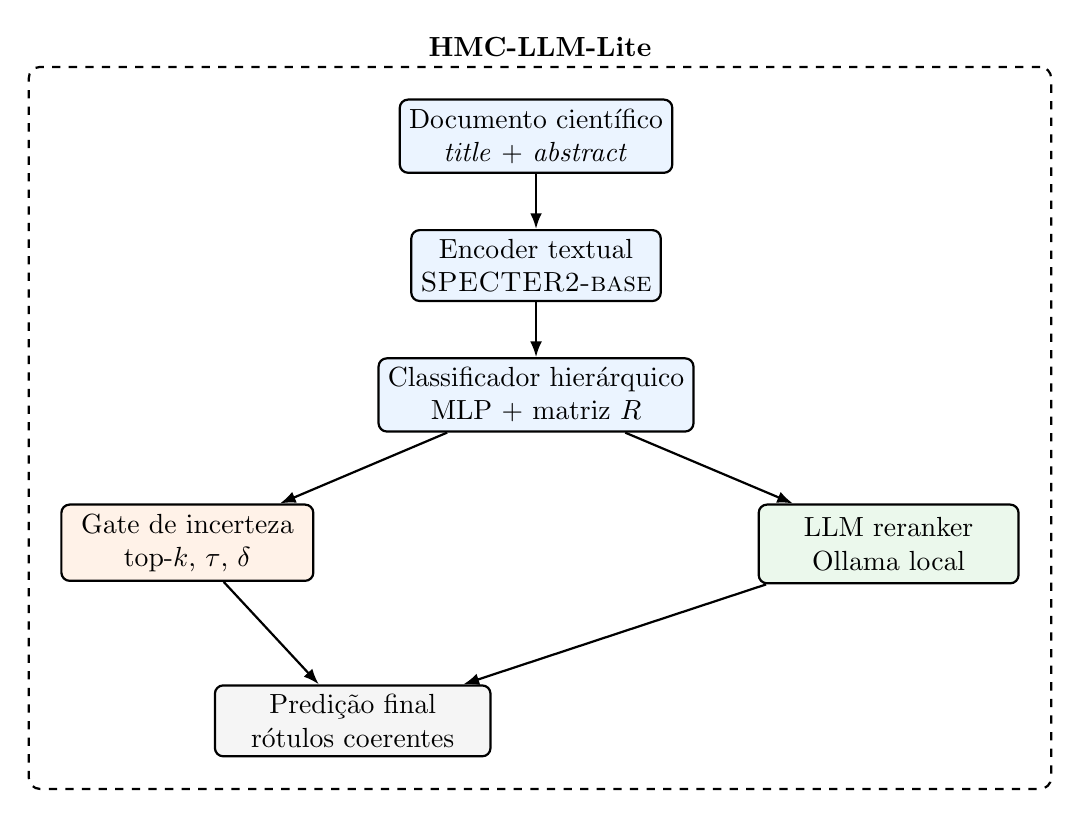
\begin{tikzpicture}[
  node distance=7mm and 13mm,
  box/.style={draw, rounded corners=3pt, thick, align=center, minimum height=9mm, minimum width=31mm, fill=softblue},
  gate/.style={draw, rounded corners=3pt, thick, align=center, minimum height=9mm, minimum width=32mm, fill=softorange},
  llm/.style={draw, rounded corners=3pt, thick, align=center, minimum height=10mm, minimum width=33mm, fill=softgreen},
  outbox/.style={draw, rounded corners=3pt, thick, align=center, minimum height=9mm, minimum width=35mm, fill=gray!8},
  arrow/.style={-{Latex[length=2mm]}, thick}
]
\node[box] (doc) {Documento científico\\\textit{title} + \textit{abstract}};
\node[box, below=of doc] (enc) {Encoder textual\\\textsc{SPECTER2-base}};
\node[box, below=of enc] (head) {Classificador hierárquico\\MLP + matriz $R$};
\node[gate, below left=9mm and 8mm of head] (gate) {Gate de incerteza\\top-$k$, $\tau$, $\delta$};
\node[llm, below right=9mm and 8mm of head] (llm) {LLM reranker\\Ollama local};
\node[outbox, below=13mm of gate, xshift=21mm] (final) {Predição final\\rótulos coerentes};

\draw[arrow] (doc) -- (enc);
\draw[arrow] (enc) -- (head);
\draw[arrow] (head) -- (gate);
\draw[arrow] (head) -- (llm);
\draw[arrow] (gate) -- (final);
\draw[arrow] (llm) -- (final);

\node[draw, dashed, rounded corners=4pt, thick, inner sep=4mm, fit=(doc)(enc)(head)(gate)(llm)(final), label={[font=\bfseries]above:\method}] {};
\end{tikzpicture}%
}
\caption{Visão geral da \method. O classificador supervisionado continua sendo
responsável por recuperar candidatos em toda a hierarquia. O LLM atua somente
como reranker sobre uma lista curta de rótulos candidatos.}
\label{fig:architecture}
\end{figure}

A Figura~\ref{fig:architecture} mostra o desenho da proposta. O pipeline começa
com um encoder científico, adequado para documentos acadêmicos. No modo atual do
\repo, o encoder padrão é \texttt{allenai/specter2\_base}; o texto de entrada é
construído a partir do título e do resumo no ArXiv, ou do resumo no WOS.

O segundo bloco é o classificador hierárquico. Na variante implementada, a base
é o modelo \texttt{globalE2E}: o transformer é ajustado junto com uma cabeça MLP,
e a saída passa pela matriz $R$ para preservar coerência entre ancestrais e
descendentes. Isso evita que o LLM precise inferir a hierarquia do zero.

O terceiro bloco é o gate de incerteza. Ele decide se a amostra deve ser enviada
ao LLM. Se o maior score já é alto e a margem para o segundo candidato é
suficiente, a predição supervisionada é aceita sem custo adicional. Caso
contrário, os top-$k$ candidatos são formatados em um prompt estruturado.

\section{Reranking por LLM}

\begin{figure}[htbp]
\centering
\resizebox{\linewidth}{!}{%
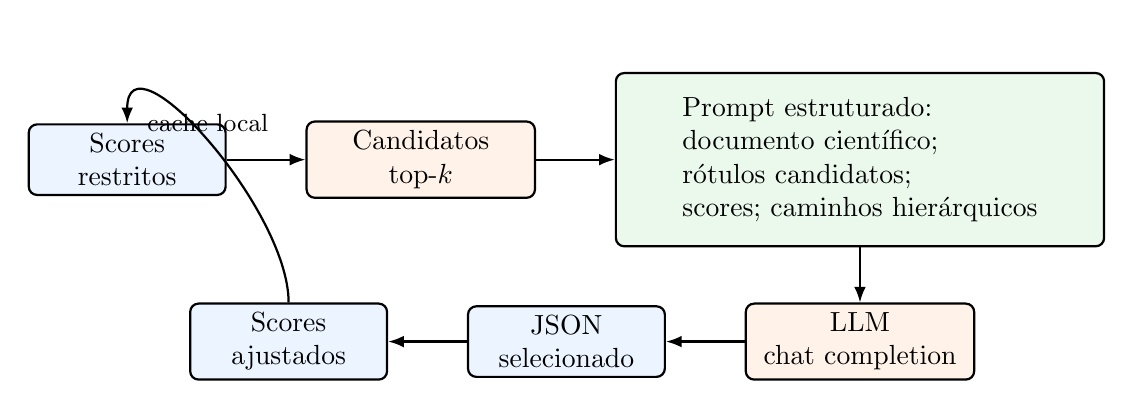
\begin{tikzpicture}[
  node distance=7mm and 10mm,
  small/.style={draw, rounded corners=3pt, thick, align=center, minimum height=8mm, minimum width=25mm, fill=softblue},
  mid/.style={draw, rounded corners=3pt, thick, align=center, minimum height=8mm, minimum width=29mm, fill=softorange},
  prompt/.style={draw, rounded corners=3pt, thick, align=left, minimum width=62mm, minimum height=22mm, fill=softgreen},
  arrow/.style={-{Latex[length=2mm]}, thick}
]
\node[small] (scores) {Scores\\restritos};
\node[mid, right=of scores] (cand) {Candidatos\\top-$k$};
\node[prompt, right=of cand] (prompt) {Prompt estruturado:\\
documento científico;\\
rótulos candidatos;\\
scores; caminhos hierárquicos};
\node[mid, below=of prompt] (api) {LLM\\chat completion};
\node[small, left=of api] (json) {JSON\\selecionado};
\node[small, left=of json] (out) {Scores\\ajustados};

\draw[arrow] (scores) -- (cand);
\draw[arrow] (cand) -- (prompt);
\draw[arrow] (prompt) -- (api);
\draw[arrow] (api) -- (json);
\draw[arrow] (json) -- (out);
\draw[arrow] (out.north) .. controls +(0,1.2) and +(0,1.2) .. node[above, font=\small]{cache local} (scores.north);
\end{tikzpicture}%
}
\caption{Detalhe do reranking. O LLM recebe apenas candidatos produzidos pelo
classificador, retorna JSON e nunca precisa gerar livremente nomes de classes.}
\label{fig:reranking}
\end{figure}

O reranking segue um contrato simples. Para cada documento incerto, o sistema
constrói uma lista de candidatos:

\begin{equation}
  c_j = (\text{label}_j, \text{score}_j, \text{path}_j).
\end{equation}

O campo \textit{path} contém o caminho hierárquico do rótulo, por exemplo
\texttt{cs > cs.LG}. O LLM recebe essa lista e deve retornar um objeto JSON com
o campo \texttt{selected\_labels}. A predição final preserva os scores dos
rótulos selecionados e zera os candidatos rejeitados:

\begin{equation}
  s'_i =
  \begin{cases}
    s_i, & \text{se } y_i \in S_{\mathrm{LLM}},\\
    0, & \text{se } y_i \in C_k(d) \setminus S_{\mathrm{LLM}},\\
    s_i, & \text{se } y_i \notin C_k(d).
  \end{cases}
\end{equation}

Essa regra é conservadora: o LLM não adiciona rótulos fora da lista proposta pelo
classificador. Ele apenas remove candidatos semanticamente fracos dentro da
lista curta. Assim, a arquitetura reduz o espaço de decisão do LLM e preserva o
aprendizado supervisionado como fonte principal de recall.

\section{Algoritmo}

O procedimento executado pela \method{} pode ser resumido da seguinte forma:

\begin{enumerate}[leftmargin=*, itemsep=3pt]
  \item Treinar o modelo base \texttt{globalE2E} com encoder científico,
        cabeça MLP e restrição hierárquica.
  \item Para cada documento de teste, calcular os scores restritos
        $\mathbf{s}=g_R(\sigma(f_\theta(d)))$.
  \item Selecionar os top-$k$ rótulos avaliáveis.
  \item Se $s_{(1)} \geq \tau$ e $s_{(1)} - s_{(2)} \geq \delta$, aceitar a
        predição do classificador.
  \item Caso contrário, enviar documento e candidatos ao LLM.
  \item Interpretar a resposta JSON e manter apenas os candidatos selecionados.
  \item Aplicar as métricas hierárquicas sobre os scores ajustados.
\end{enumerate}

Na implementação do \repo, esse procedimento é exposto pelo argumento:

\begin{verbatim}
python -m hmc.main \
  --dataset_name arxiv \
  --method globalLLMLite \
  --device cuda \
  --dataset_path ./data \
  --output_path ./output
\end{verbatim}

\section{Diferença para uso direto de LLM}

Uma alternativa simples seria pedir ao LLM que classifique diretamente cada
documento dentro da taxonomia. Essa opção é menos controlada por três motivos.
Primeiro, o LLM precisaria considerar dezenas ou centenas de rótulos em cada
chamada. Segundo, a resposta poderia conter classes inexistentes, nomes
parafraseados ou níveis incompletos da hierarquia. Terceiro, o custo cresceria
linearmente com o número de documentos, mesmo nos casos em que o classificador
supervisionado já está confiante.

A \method{} evita esses problemas ao decompor a decisão. O classificador neural
faz a recuperação ampla e barata. O LLM entra apenas como árbitro local em
regiões ambíguas do espaço de rótulos. Essa separação é especialmente adequada
para taxonomias científicas, onde muitas confusões relevantes ocorrem entre
subáreas próximas, como aprendizado de máquina, inteligência artificial,
estatística computacional e otimização.

\section{Implementação}

A implementação atual é composta por três módulos principais:

\begin{table}[htbp]
\centering
\begin{tabular}{lll}
\toprule
\textbf{Componente} & \textbf{Arquivo} & \textbf{Função} \\
\midrule
Entrada principal & \texttt{src/hmc/main.py} & Seleciona \texttt{globalLLMLite} \\
Pipeline LLM & \texttt{llm\_train.py} & Treina E2E e aplica postprocess \\
Cliente Ollama & \texttt{ollama\_agent.py} & Prompt, chamada local e parse JSON \\
\bottomrule
\end{tabular}
\caption{Componentes da implementação da \method{} no \repo.}
\label{tab:implementation}
\end{table}

O modo \texttt{globalLLMLite} chama internamente o treinamento
\texttt{globalLLM}, mas fixa uma política mais econômica: o reranking é aplicado
apenas a amostras incertas e a resposta do LLM é curta. Os principais parâmetros
são \texttt{llm\_top\_k}, \texttt{llm\_margin},
\texttt{llm\_confidence\_threshold}, \texttt{llm\_max\_tokens},
\texttt{llm\_temperature}, \texttt{llm\_k\_max},
\texttt{llm\_expand\_hierarchy}, \texttt{llm\_max\_calls},
\texttt{llm\_timeout}, \texttt{llm\_base\_url} e \texttt{llm\_num\_ctx}.
O modelo padrão de LLM é configurável; no código atual, o valor inicial é
\texttt{qwen3:14b}.

A chamada ao LLM é executada diretamente contra o endpoint local do Ollama. O
cliente não usa cache, rotação de chaves ou fallback silencioso para a predição
base: falhas de comunicação ou respostas inválidas interrompem o experimento.
As estatísticas do reranking são salvas junto com o arquivo
\texttt{test-scores.json}, incluindo número de chamadas, amostras ignoradas por
confiança e \textit{recall@k} dos candidatos.

\section{Protocolo experimental sugerido}

A avaliação deve comparar a \method{} contra três baselines do próprio
repositório:

\begin{enumerate}[leftmargin=*, itemsep=2pt]
  \item \texttt{global}: encoder congelado, embeddings pré-computados e MLP com
        restrição hierárquica.
  \item \texttt{globalE2E}: ajuste end-to-end do transformer com cabeça global.
  \item \texttt{globalSOTA}: transformer ajustado com GNN sobre o grafo de
        rótulos.
\end{enumerate}

As métricas principais devem incluir Micro-F1, Macro-F1, precisão e recall por
nível hierárquico. Também é necessário reportar métricas operacionais:
percentual de documentos enviados ao LLM, número total de chamadas, custo
estimado, latência média e taxa de respostas inválidas ou vazias.
Para evitar otimização direta no conjunto de teste, o protocolo do artigo usa
limiar fixo de decisão em $0{,}5$ por padrão; a busca por melhor limiar deve ser
mantida desativada, exceto em ablações explicitamente identificadas.

\begin{table}[htbp]
\centering
\begin{tabular}{llll}
\toprule
\textbf{Método} & \textbf{Encoder} & \textbf{Hierarquia} & \textbf{LLM} \\
\midrule
\texttt{global} & Congelado & Matriz $R$ & Não \\
\texttt{globalE2E} & Ajustado & Matriz $R$ & Não \\
\texttt{globalSOTA} & Ajustado & Matriz $R$ + GNN & Não \\
\texttt{globalLLMLite} & Ajustado & Matriz $R$ & Gate incerto \\
\bottomrule
\end{tabular}
\caption{Comparação entre regimes experimentais no \repo.}
\label{tab:methods}
\end{table}

\section{Hipóteses}

A proposta deve ser avaliada a partir de três hipóteses:

\begin{enumerate}[leftmargin=*, itemsep=2pt]
  \item \textbf{H1:} o reranking melhora a precisão em rótulos folha, pois remove
        candidatos semanticamente plausíveis mas incorretos.
  \item \textbf{H2:} o ganho é maior em documentos incertos, isto é, quando a
        margem entre os principais candidatos é pequena.
  \item \textbf{H3:} o custo permanece controlado porque apenas uma fração dos
        documentos aciona o LLM.
\end{enumerate}

Essas hipóteses também indicam os riscos. Um LLM muito conservador pode aumentar
precisão e reduzir recall. Um gate muito agressivo pode enviar documentos demais
ao LLM e tornar o método caro. Por isso, $\tau$, $\delta$ e $k$ devem ser tratados
como hiperparâmetros, não como constantes universais.

\section{Limitações e mitigações}

As limitações principais da \method{} podem ser tratadas dentro da própria
arquitetura. A primeira é a dependência do top-$k$: se o rótulo correto não entra
na lista de candidatos, o LLM não consegue selecioná-lo. Para reduzir esse risco,
o gate passa a usar uma seleção adaptativa em vez de um $k$ fixo. Em documentos
de baixa confiança, o sistema expande a lista até $k_{\max}$ e inclui também
rótulos estruturalmente próximos: pais, filhos e irmãos dos candidatos mais bem
pontuados. Assim, o LLM continua operando sobre um espaço pequeno, mas com maior
chance de conter a classe correta.

\begin{equation}
  C(d)=\operatorname{TopK}(\mathbf{s}, k(d)) \cup
  \operatorname{Anc}(C) \cup \operatorname{Child}(C) \cup \operatorname{Sib}(C),
\end{equation}

\noindent onde $k(d)$ cresce com a incerteza do classificador e é limitado por
$k_{\max}$. Na avaliação, esse mecanismo deve ser acompanhado pela métrica
\textit{recall@k} dos candidatos, pois ela mede se o gargalo está no recuperador
neural ou no reranker.

A segunda limitação envolve custo, latência e dependência de um provedor externo.
Ela é mitigada por quatro mecanismos: chamadas apenas para amostras incertas,
cache determinístico por conteúdo do prompt, \textit{fallback} automático para a
predição supervisionada em caso de erro ou timeout, e orçamento máximo de
chamadas por execução. Com isso, o LLM deixa de ser uma dependência crítica do
pipeline: quando a chamada falha, o sistema mantém a saída do classificador base.

\begin{table}[htbp]
\centering
\begin{tabular}{lll}
\toprule
\textbf{Risco} & \textbf{Mitigação} & \textbf{Efeito esperado} \\
\midrule
Rótulo fora do top-$k$ & Top-$k$ adaptativo + vizinhança hierárquica & Maior recall de candidatos \\
Custo elevado & Gate de incerteza + cache & Menos chamadas externas \\
Latência & Cache + limite de chamadas & Tempo controlado por execução \\
Resposta inválida & Validação JSON + fallback & Robustez operacional \\
Variação do provedor & Modelo versionado + cache congelado & Reprodutibilidade \\
\bottomrule
\end{tabular}
\caption{Mitigações incorporadas à proposta para tornar o uso de LLM controlado
e reprodutível.}
\label{tab:mitigations}
\end{table}

A terceira limitação é que o reranking, isoladamente, atua apenas no
pós-processamento. A solução proposta é transformar as decisões do LLM em sinal
fraco de treinamento. As respostas aceitas podem alimentar um conjunto auxiliar
de pares positivos e negativos: candidatos selecionados pelo LLM são tratados
como positivos, enquanto candidatos rejeitados dentro do mesmo top-$k$ são
tratados como negativos difíceis. Esse conjunto permite treinar um reranker local
menor ou calibrar os limiares $\tau$ e $\delta$ sem depender do LLM em todas as
execuções futuras.

Para o primeiro experimento, a arquitetura opera no modo \textbf{online}: o LLM
é usado diretamente no pós-processamento das amostras incertas. Como extensão
posterior, o histórico de decisões do LLM pode alimentar um modo
\textbf{destilado}, no qual um módulo local de calibração aproxima o
comportamento do reranker externo e reduz chamadas em rodadas futuras. Essa
estratégia preserva o ganho semântico do LLM, mas move parte do custo para uma
etapa offline e reaproveitável.

\section{Conclusão}

Este artigo apresentou a \method, uma proposta de arquitetura para classificação
hierárquica de documentos científicos que combina aprendizado supervisionado com
reranking semântico por LLM. O desenho preserva o classificador neural como
mecanismo principal de recuperação e usa o LLM apenas em casos incertos, sobre
um conjunto restrito de candidatos válidos. Essa escolha busca capturar o melhor
dos dois regimes: eficiência e cobertura do classificador, interpretação
semântica local do LLM e coerência estrutural da matriz hierárquica.

No contexto do \repo, a proposta é implementada pelo método
\texttt{globalLLMLite} e pode ser avaliada diretamente nos datasets ArXiv e WOS.
Com as mitigações propostas, o método deixa de depender de um top-$k$ rígido,
controla custo por gate e cache, mantém fallback determinístico para falhas
externas e cria um caminho de destilação para reaproveitar decisões do LLM no
treinamento futuro. O primeiro experimento deve medir simultaneamente ganho de
F1, recall@k dos candidatos, redução de erros em rótulos folha e custo médio por
documento.

\section*{Referências}

\begin{enumerate}[leftmargin=*, itemsep=2pt]
  \item Cohan, A. et al. \textit{SPECTER: Document-level Representation Learning
        using Citation-informed Transformers}. ACL, 2020.
  \item Giunchiglia, E. and Lukasiewicz, T. \textit{Coherent Hierarchical
        Multi-label Classification Networks}. NeurIPS, 2020.
  \item Zhou, J. et al. \textit{Hierarchy-Aware Global Model for Hierarchical
        Text Classification}. ACL, 2020.
  \item Wang, Z. et al. \textit{Incorporating Hierarchy into Text Encoder: a
        Contrastive Learning Approach for Hierarchical Text Classification}.
        ACL, 2022.
  \item Wang, Z. et al. \textit{HPT: Hierarchy-aware Prompt Tuning for
        Hierarchical Text Classification}. EMNLP, 2022.
\end{enumerate}

\end{document}
